\section{The price of a new distinction}
\label{section:the-price-of-a-shared-description}

Suppose two computations use the same stored parameter $q\in\mathbb R^2$. One prefers $a=(1,0)$ and the other prefers $b=(\cos\theta,\sin\theta)$. Their losses are
\begin{equation}
 \ell_1(q)=\tfrac12\|q-a\|^2,\qquad
 \ell_2(q)=\tfrac12\|q-b\|^2,\qquad
 d^2=\|a-b\|^2=2(1-\cos\theta).
 \label{eq:register-losses}
\end{equation}
We take $0\leq\theta\leq\pi$. Here $\theta$ measures disagreement between the tasks and $d$ is the distance between their preferred settings. Neither task is difficult on its own. The difficulty comes from asking one register to serve both.

Give the first task weight $\alpha$ and the second weight $1-\alpha$, with $0\leq\alpha\leq1$. Completing the square gives
\begin{equation}
 \alpha\ell_1+(1-\alpha)\ell_2
 =\tfrac12\|q-q_*\|^2+\tfrac12\alpha(1-\alpha)d^2,
 \qquad q_*=\alpha a+(1-\alpha)b.
 \label{eq:register-square}
\end{equation}
The first term can be removed by optimisation. The second cannot: it is the price of the compromise within this representation. At equal weights it is $d^2/8$. If maintaining a second register costs an additional $c$, separate descriptions are preferable when $c<d^2/8$. The relevant comparison is between the total costs of two ways of performing the same pair of tasks, not between their storage sizes in isolation.

\emph{Self-Consistent Loss Geometries}~\cite{McCaulda239a} develops a coupled-evaluator model in which the system can also change the attention paid to each task. It adds a conflict charge $\gamma\alpha(1-\alpha)d^2$ and an arbitration penalty $2\eta(\alpha-\tfrac12)^2$. The parameters $\gamma\geq0$ and $\eta>0$ specify those modelled costs. The second penalty makes ignoring a task costly. After optimising $q$ and $\alpha$, the fixed shared-register model has
\begin{equation}
 L_B^*=\min\left\{\frac{d^2}{4}\left(\tfrac12+\gamma\right),
                         \frac{\eta}{2}\right\}.
 \label{eq:shared-optimum}
\end{equation}
Its options are balanced compromise or suppression of one evaluator. In the split option each task has its own minimising coordinate, removing the disagreement penalty by construction. The remaining incremental partition cost is $C_{\rm part}\geq0$, so the system achieves
\begin{equation}
 L_C^*=\min\{L_B^*,C_{\rm part}\}.
 \label{eq:partition-optimum}
\end{equation}
Figure~\ref{fig:dd-shared-register-price} makes the choice visible. At the stated register price, splitting becomes favourable before the fixed shared representation would suppress an evaluator. The useful adaptation is a change in what the register distinguishes.
\begin{figure}[htbp]
\centering
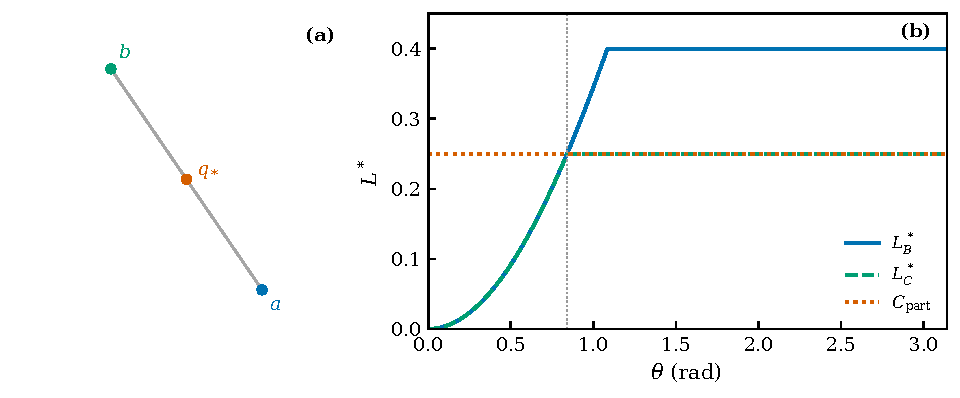
\includegraphics[width=\linewidth]{figures/portable-run-b69220b3a27348ad.result/dd-shared-register-price.pdf}
\caption{When should two tasks stop sharing a register? (a) The equally weighted quadratic compromise is $q_*=(a+b)/2$. (b) Fixed-register loss $L_B^*$ and partition-enabled loss $L_C^*$ versus disagreement angle $\theta$, for $\gamma=1$, $\eta=0.8$ and $C_{\rm part}=0.25$. Splitting becomes cheaper at $\theta=0.8411$ radians, before the fixed-register model suppresses an evaluator at $1.0853$. The curves evaluate the classical cost model in Eqs.~\eqref{eq:shared-optimum}--\eqref{eq:partition-optimum}.}
\label{fig:dd-shared-register-price}
\end{figure}

The classical model turns representation choice into an ordinary optimisation: tolerate the compromise or pay to remove it. The same question will recur in the quantum and memory examples: when should additional capacity buy a new distinction rather than more work inside the existing description?
\subsection{When a second register is worth its price}
Varying the register price as well as the disagreement reveals three regimes, shown in Figure~\ref{fig:dd-register-phase-diagram}. The boundary follows directly from the same objective. Write $A(\theta)=(\tfrac12+\gamma)d^2$. After minimising the shared coordinate, its remaining attention cost is
\[
 \frac{A(\theta)}4+\bigl(2\eta-A(\theta)\bigr)
                   \left(\alpha-\tfrac12\right)^2.
\]
Balanced sharing is therefore optimal when $A<2\eta$, while the shared model suppresses one evaluator when $A>2\eta$. Allowing the register itself to split gives the short result
\begin{equation}
 L_*=\min\left\{C_{\rm part},\frac{A(\theta)}4,\frac{\eta}2\right\},
 \qquad
 C_{\rm crit}(\theta)=
 \min\left\{\frac{\tfrac12+\gamma}{2}(1-\cos\theta),\frac{\eta}2\right\}.
 \label{eq:register-phase-boundary}
\end{equation}
For $C_{\rm part}<C_{\rm crit}$, two registers are preferable. Above the boundary, one is cheaper. Equality gives tied representations. The optimal cost is continuous across the share--split boundary, but generically has a kink as the preferred number of registers changes. This is an optimisation phase transition in a finite model.

At $A=2\eta$, every shared attention weight is degenerate. This boundary is reachable for $0\leq\theta\leq\pi$ when $\eta\leq2(\tfrac12+\gamma)$. The flat part of the boundary is informative. Once conflict is sufficiently large, the shared model can pay $\eta/2$ to abandon an evaluator instead of buying a second register. With $\gamma=1$ and $\eta=0.8$, the three regions meet at $\theta_{\rm att}=\arccos(1-\eta/(\tfrac12+\gamma))\simeq1.0853$ and $C_{\rm part}=0.4$. The earlier $C_{\rm part}=0.25$ example is a horizontal slice: increasing disagreement crosses from balanced sharing to separate registers at $\theta_{\rm split}\simeq0.8411$. The diagram makes the design choice explicit - tolerate a compromise, pay for another distinction, or sacrifice one of the tasks.

\begin{figure}[htbp]
\centering
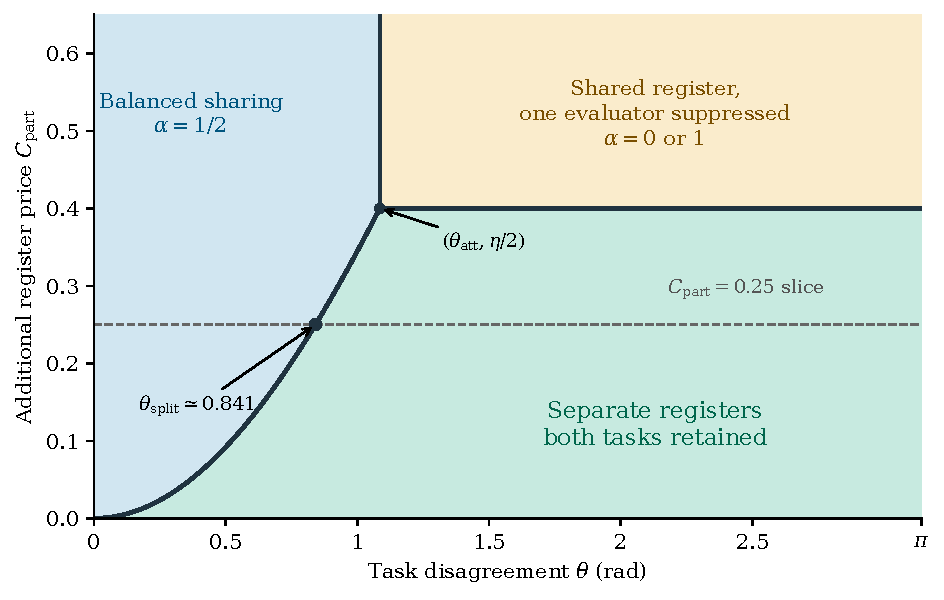
\includegraphics[width=0.93\linewidth]{figures/phase-run-939b6a8b76724d02.result/dd-register-phase-diagram.pdf}
\caption{The register-choice phase diagram for $\gamma=1$ and $\eta=0.8$. Below $C_{\rm crit}(\theta)$, splitting retains both tasks. Above it, the shared optimum is balanced at small $\theta$ and suppresses an evaluator at large $\theta$. Solid boundaries mark tied costs, including the vertical attention boundary above the meeting point. At that meeting point all shared attention weights are degenerate and splitting has the same cost. The dashed $C_{\rm part}=0.25$ slice recovers Figure~\ref{fig:dd-shared-register-price}. The regions are the exact optima of the declared finite model.}
\label{fig:dd-register-phase-diagram}
\end{figure}

\subsection{A cost coordinate and a task}\label{subsec:cost-task}
The register example assumes a price for an extra description. A separate question is how to choose a cost coordinate when independent capacities compose. \emph{The Cost of Complexity} and \emph{Foundations of Synthetics} motivate a logarithmic coordinate from multiplicative capacity and additive cost.~\cite{Reference975536} If independent capacities $M$ and $N$ compose multiplicatively, while their costs add, a nondecreasing cost function obeying $f(MN)=f(M)+f(N)$ has the form $f(N)=\kappa\log N$. The scale $\kappa\geq0$ fixes the cost unit. The premise concerns the capacity or product-order count being composed. A single globally sorted probability rank is a different object and need not multiply. This distinction matters: forcing two partially ordered descriptions into one global list can introduce comparisons that neither task required.

For fixed labels $r=1,\ldots,R$ with cost $\log r$, maximum entropy chooses the least concentrated probability law compatible with a specified mean cost. The partition sum below normalises those probabilities. The resulting family is
\begin{equation}
 p_\lambda(r)=\frac{r^{-\lambda}}{Z_R(\lambda)},\qquad
 Z_R(\lambda)=\sum_{r=1}^{R}r^{-\lambda}.
 \label{eq:cost-family}
\end{equation}
The multiplier $\lambda$ is the price conjugate to mean log-cost. Increasing it concentrates probability on cheaper labels. If $C_R=\sum_r p_\lambda(r)\log r$, then
\begin{equation}
 C_R=-\partial_\lambda\log Z_R,\qquad
 -\frac{dC_R}{d\lambda}
 =\operatorname{Var}_{p_\lambda}(\log r)
 =g_{\lambda\lambda}.
 \label{eq:cost-geometry}
\end{equation}
The response coefficient measures how distinguishable nearby probability laws are. It is also the Fisher information of this same one-parameter family, obtained by averaging $(\partial_\lambda\log p_\lambda)^2$. Thus cost response and statistical distinguishability are two readings of one construction. For a small change $\delta\lambda$, the relative entropy is
$D(p_\lambda\|p_{\lambda+\delta\lambda})
=\tfrac12g_{\lambda\lambda}(\delta\lambda)^2+O((\delta\lambda)^3)$.
This is a specific bridge from a cost coordinate to geometry, with the underlying probability distribution held in view. Calibrating $C_{\rm part}$ in seconds, joules or bytes is a further application-level task: the representational price must be connected to the resources and prediction error that matter.

At finite $R$ these expressions are smooth. The infinite counting-measure model has $Z_\infty(\lambda)=\zeta(\lambda)$ only for $\lambda>1$, and becomes singular at its normalisability boundary. This distinguishes a singular infinite limit from the smooth finite models. Physical heat, in turn, is charged to an operation on an ensemble. Landauer's reset analysis concerns the effect of a specified erasure protocol on information-bearing physical states.\footnote{R. Landauer, \emph{Irreversibility and Heat Generation in the Computing Process}, IBM Journal of Research and Development 5 (1961), \href{https://doi.org/10.1147/rd.53.0183}{doi:10.1147/rd.53.0183}.} Foundations makes this distinction concrete using retained side information and explicit bath/register operations.~\cite{Landauer1961f2ecf4}

A task supplies the other half of the accounting. Let $\Omega$ denote the underlying situation, $X$ its retained description and $Y$ the quantity to be predicted. For an encoder with $Y$ conditionally independent of $X$ given $\Omega$, and a decoder distribution $q(Y|X)$, the expected logarithmic prediction loss separates as
\begin{equation}
 \mathbb E[-\log q(Y|X)]
 =H(Y|\Omega)+I(Y;\Omega|X)
   +\mathbb E_X D\!\left(P(Y|X)\|q(Y|X)\right).
 \label{eq:predictive-loss}
\end{equation}
Here $H$ is the uncertainty left after the stated condition is known. The conditional mutual information $I(Y;\Omega|X)$ measures the predictive information about $Y$ available in $\Omega$ but absent from $X$. Relative entropy is $D(p\Vert q)=\sum_y p(y)\log[p(y)/q(y)]$: the excess expected logarithmic prediction loss from using $q$ when the outcomes follow $p$. The three terms are the target's intrinsic uncertainty, the predictive information lost by the encoder, and the decoder's mismatch. Better decoding cannot recover a distinction that was discarded. A larger description cannot remove randomness already present in the target.

Foundations illustrates this with three input bits $(a,b,c)$. The bit $c$ labels a sensor but does not affect the alarm probability. For $(a,b)=(00,01,10,11)$ those probabilities are $0.1,0.3,0.7,0.9$. Retaining $(a,b)$ preserves the forecasts exactly while discarding $c$. Retaining only $a$ gives the coarser forecasts $0.2$ and $0.8$ under the declared uniform input law. The adequate representation depends on the prediction being requested, not on preserving every input bit.

The next distinction can also have a local value. With a false stop costing one unit and a missed alarm three, the optimal alarm threshold is probability $1/4$. After observing $a=0$, acquiring $b$ reduces conditional decision risk from $0.6$ to $0.5$. After $a=1$, it does not change the preferred action. At acquisition cost $k<0.1$, buying $b$ only on the first branch improves total expected cost from $0.40$ to $0.35+0.5k$. Uniformly increasing resolution would pay for information where it changes nothing.

This also explains why a purely greedy refinement rule can be inadequate. A local step may cost more than its immediate benefit but unlock a valuable later calculation. For a finite refinement tree, an incremental gain $a_v$ at node $v$ and conditional child probabilities $q(u|v)$ give the backward recursion
\begin{equation}
 V(v)=\max\left\{0,\ a_v+\sum_u q(u|v)V(u)\right\}.
 \label{eq:refinement-value}
\end{equation}
A step with immediate gain $-1$ can be worthwhile if it unlocks gain $5$ with probability $0.6$: its continuation value is $2$. Efficient representation is a policy for purchasing the distinctions and intermediate constructions that make useful work possible. When the task is to predict an evolving process, the value of a distinction depends on what it lets us say about the future. A summary that answers today's question may not contain enough information to answer tomorrow's.

